\documentclass{article}

\usepackage{url}
\usepackage[hmargin=1.5in]{geometry}
\usepackage{amsmath}
\usepackage{amssymb}
\usepackage{amsthm}
%\usepackage{eqnarray}
\usepackage{stmaryrd} %% needed for mapsto arrows in commutative diagrams
\usepackage{bm} %% for putting series names in bold
%%\usepackage{amsthm}
\usepackage{graphicx}
\usepackage{fancyhdr}
\usepackage{enumitem}
\usepackage[svgnames]{xcolor} %% for revisions
\usepackage{xparse} %% for squiggly underlines
\usepackage{tikz-cd} %% for term norm scratch work
\usepackage{tikz}
%\usepackage{eqnarray}

\let\Re\relax
\DeclareMathOperator{\Re}{Re}
\let\Im\relax
\DeclareMathOperator{\Im}{Im}

\usetikzlibrary{bbox}
\usetikzlibrary{fadings}

\pgfdeclareradialshading{radialedge}{\pgfpointorigin}{%
  color(0bp)=(transparent!0);
  color(20bp)=(transparent!0);
  color(22bp)=(transparent!10);
  color(24bp)=(transparent!90);
  color(25bp)=(transparent!100)
}
\pgfdeclarefading{radial edge}{\pgfuseshading{radialedge}}%

% function spaces
\newcommand{\cont}{\mathcal{C}}
\newcommand{\holo}{\mathcal{H}}
\newcommand{\singexp}[2]{\mathcal{H}L^\infty_{#1, #2}}
\newcommand{\singexpalg}[1]{\singexp{#1}{\bullet}}
\newcommand{\dualsingexp}[2]{\widehat{\mathcal{H}}L^\infty_{#1, #2}}
\newcommand{\dualsingexpalg}[1]{\singexp{#1}{\bullet}}
\newcommand{\holoL}[1]{\mathcal{H}L^{#1}} %% remove once we stop using old arguments

%% editing
\newcommand{\done}[1]{\textcolor{gray}{#1}}

\theoremstyle{definition}
\newtheorem{defn}{Definition}
%%\theoremstyle{plain}
%%\newtheorem{prop}{Proposition}

% convenience aliases
\newcommand{\maps}{\colon}
\newcommand{\acts}{\mathbin{\raisebox{\depth}{\rotatebox{-90}{$\circlearrowright$}}}}


% symbology
\newcommand{\Z}{\mathbb{Z}}
\newcommand{\R}{\mathbb{R}}
\newcommand{\C}{\mathbb{C}}
\newcommand{\Q}{\mathbb{Q}}
\usepackage{tikz}
\usepackage{tikz-cd}
\usepackage{rotating}
\newcommand*{\isoarrow}[1]{\arrow[#1,"\rotatebox{90}{\(\sim\)}"
]}

\newcommand{\series}[1]{\tilde{#1}}
\newcommand{\fracderiv}[3]{\partial^{#1}_{#2, #3}}
\newcommand{\blankbox}{{\fboxsep 0pt \colorbox{lightgray}{\phantom{$h$}}}}
\newcommand{\laplacepde}{\mathcal{D}}
\newcommand{\van}{\mathfrak{m}}
\DeclareMathOperator{\Ai}{Ai}
\usetikzlibrary{matrix,shapes,arrows,decorations.pathmorphing}
\tikzset{commutative diagrams/arrow style=math font}
\tikzset{commutative diagrams/.cd,
mysymbol/.style={start anchor=center,end anchor=center,draw=none}}
\newcommand\MySymb[2][\square]{%
  \arrow[mysymbol]{#2}[description]{#1}}
\tikzset{
shift up/.style={
to path={([yshift=#1]\tikztostart.east) -- ([yshift=#1]\tikztotarget.west) \tikztonodes}
}
}
\DeclareMathAlphabet{\mathpzc}{OT1}{pzc}{m}{it}

\newcommand*{\defeq}{\mathrel{\vcenter{\baselineskip0.5ex \lineskiplimit0pt
                     \hbox{\scriptsize.}\hbox{\scriptsize.}}}%
                     =}
\newcommand*{\defeqin}{\mathrel{\vcenter{\lineskiplimit0pt\baselineskip0.5ex
                     \hbox{\scriptsize.}\hbox{\scriptsize.}}}%
                     =}                     

%%\let\Re\relax
%%\DeclareMathOperator{\Re}{Re}

\newcommand{\laplace}{\mathcal{L}}
\newcommand{\borel}{\mathcal{B}}
\newcommand{\aexp}{\text{\ae}}
\newcommand{\deriv}[3]{\partial^{#1}_{#2 \text{ from } #3}}


\newtheorem{definition}{Definition}[section]
\newtheorem{remark}[definition]{Remark}
\theoremstyle{plain}
\newtheorem{theorem}{Theorem}[section]
\newtheorem{prop}[definition]{Proposition}
\newtheorem{corollary}[theorem]{Corollary}
\newtheorem{lemma}[definition]{Lemma}
%\newtheorem{conjecture}[definition]{Conjecture}
\newtheorem{claim}[definition]{Claim}
%\newtheorem{exercise}[definition]{Exercise}
\newtheorem*{notation*}{Notation}

% drafting environments
\newenvironment{verify}{\color{ForestGreen}}{\color{black}}
\newenvironment{brainstorm}{\color{violet}\begin{itemize}}{\end{itemize}\color{black}}

% colors
\definecolor{ietocean}{RGB}{0, 30, 140}
\definecolor{ietcoast}{RGB}{0, 150, 173}
\definecolor{ietlagoon}{RGB}{0, 216, 180}

% pretty prince hyperref must always be the last thing in the preamble, always
\usepackage{hyperref}
\hypersetup{
  colorlinks,
  linkcolor={ietcoast},
  citecolor={ietcoast},
  urlcolor={ietcoast}
}

\setcounter{tocdepth}{2}

\title{Geometry of thimble integrals}
\author{Veronica Fantini}

\begin{document}
\maketitle



\section{Geometry of thimble integrals}\label{apx:geometry_thimble_integrals}

Let $X$ be an $N$-dimensional complex algebraic variety and $f\colon X\to\C$ a proper algebraic map with non-degenerate critical points $a_1,...,a_N$ and critical values $\alpha_j=f(a_j)$\footnote{Everything we’ll discuss, applies also when $X$ is a $N$-dimensional complex (K\"ahler) manifold and $f\colon X\to\C$ is a holomorphic function with non-degenerates critical points, which is, for example, the setting in \cite{Witten}.}: for a fixed $z\in\C$, we are interested in integrals of the form 
\[
I(z):=\int_{\mathcal{C}}e^{-zf}\nu
\]
regarded as holomorphic functions on the frequency domain for a suitable choice of a contour $\mathcal{C}$ and an $N$-form $\nu$. In fact, we'll introduce homology and cohomology groups $H_{*}^{B,z}$ and $H_{dR,z}^*$ for which the function $I(z)$ will represent the Poincar\'e pairing. 

We begin with the definition of $H_{*}^{B,z}$: it is the relative homology group with respect to $zf$, and its definition requires some preliminaries. We follow \cite{pham} and \cite[Section 1]{Arnold}. Let us fix $z\in\C$ and $\theta=\arg z$; for every $c>0$ we define 
\begin{align*}
    S_c^+(\theta) &:=\lbrace \zeta\in\C \vert \Re (\zeta e^{i\theta})\geq c \rbrace\\
    S_c^-(\theta)&:=\lbrace \zeta\in\C \vert \Re (\zeta e^{i\theta})\leq c \rbrace
\end{align*}
and $H_{*}^{B,z}:=H_{*}(X,f^{-1}(S_c^+(\theta)))$ for $c$ large enough\footnote{In fact $H_{*}^{B,z}$ is defined after taking the projective limit $c\to\infty$ of the chain complex with support $\{A\subset X \text{ closed s.t. } \forall c>0 f^{-1}(S_c^-(\theta))\cup A \text{ is compact }  \}$.}. Moreover, $H_n(X,f^{-1}(S_c^+(\theta)))$ can be identified with the homology of a generic fiber $H_{n-1}(f^{-1}(p_0))$ with $p_0\neq \{\alpha_j\}$. This leads to further identifications:

\begin{equation}
    H_{*}^{B,z}\cong \bigoplus_{\alpha_i} H_{*}(B_j, B_j^+(\theta))
\end{equation}
where $B_j:=f^{-1}(B_r(\alpha_j))$ is the preimage of a small ball or radius $r$, containing only the critical value $\alpha_i$ and $B_j^+(\theta):=f^{-1}\left(B_r(\alpha_j)\cap \{ \Re (\zeta e^{i\theta})\geq r/2\}\right)$. Notice that we are not assuming $f$ to be Morse, hence $B_j$ may have different connected components. Then 

\begin{equation}
    H_{n}(B_j, B_j^+(\theta))\cong H_{n-1}(f^{-1}(p_j))\cong \begin{cases} \Z^{\mu_j} & \text{if } n=N\\
     0 & \text{otherwise}
    \end{cases}
\end{equation}
where $|p_j-\alpha_j|=r$, $\Re(p_j e^{i\theta})=r$, and $\mu_j$ is a number in $\{\textcolor{magenta}{???}\}$ called the {\em Milnor number} of the critical \textcolor{red}{point/value $a_j/\alpha_j$}. 


\begin{center}
    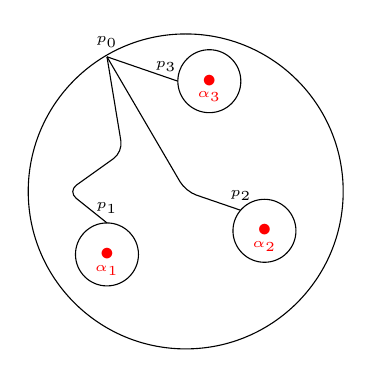
\begin{tikzpicture}
        \draw (2,2) circle (2);
        \node[font=\tiny,red] at (1,1) {$\alpha_1$};
        \draw (1,1.2) circle (0.4);
        \node[font=\tiny,red] at (3,1.3) {$\alpha_2$};
        \draw (3,1.5) circle (0.4);
        \node[font=\tiny,red] at (2.3,3.2) {$\alpha_3$};
        \draw (2.3,3.4) circle (0.4);
        \node[above,red] at (1,1) {$\bullet$};
        \node[above,red] at (3,1.3) {$\bullet$};
        \node[above,red] at (2.3,3.2) {$\bullet$};
        \draw[rounded corners] (2.7,1.76)--(2,2)--(1,3.71);
        \draw[rounded corners] (1,1.6)--(0.5,2)--(1.2,2.5)--(1,3.71);
        \draw[rounded corners] (1.9,3.4)--(1,3.71);
        \node[font=\tiny, above] at (1,3.71) {$p_0$};
        \node[font=\tiny, above] at (2.7,1.76) {$p_2$};
        \node[font=\tiny, above] at (1,1.6) {$p_1$};
        \node[font=\tiny, above] at (1.75,3.4) {$p_3$};
    \end{tikzpicture}
\end{center}

From the classical theory of singularities \cite[\textcolor{magenta}{add section; move to end of sentence}]{Arnold}, we know that $H_{N-1}(f^{-1}(p_0))$ has a distinguished basis of \textit{vanishing cycles} from the generic fiber over $p_0$ to the preimage of each critical value. Each vanishing cycle is represented by the boundary of a so-called \textit{Lefschetz thimble}: since we assumed critical points to be non--degenerate, in a neighborhood of $a_j$ there are local coordinates $x_1,...,x_N$ such that 
\[f=\alpha_j+\sum_{k=1}^N x_k^2\]

and for $p=c e^{i\theta}\in\C$, the thimble $\Lambda_j(p)$ is defined by 
\begin{align*}
    \Im(x_1)=...=\Im(x_N)=0 \text{ and } \Re(e^{-i\theta/2}x_1)^2+....+\Re(e^{-i\theta/2}x_N)^2\leq c
\end{align*}
Equivalently, Lefschetz thimbles are gradient flow trajectories departing from the critical points of $f$ (see \cite[page~10]{Witten}).

Hence we deduce that $H_{z, N}^B$ admits a distinguished basis of Lefschetz thimbles labeled by critical points.


Then we recall the definition of $H_{dR,z}^*$: it is the hypercohomolgy of the twisted de Rham complex 

\begin{equation*}
    H_{dR,z}^*:=\mathbb{H}^*( \Omega^\bullet(X), zd+df)
\end{equation*}
where $(\Omega^\bullet(X), d)$ is the de Rham complex of differential forms on $X$. 

Therefore, the integral $I(z)$ can e regarded as the image of the following map: 

\begin{align*}
    \int \colon  H_{z,N}^{B} \times & H_{dR,z}^N \to \C \\
       [\mathcal{C}] ,\,\, & [\nu] \to \int_{\mathcal{C}}e^{-zf}\nu
\end{align*}

\textcolor{orange}{[the Betti--de Rham isomorphism is necessary?]}

Since every cycle $\mathcal{C}$ can be written as a linear combination of Lefschetz thimbles, we restrict our attention to  \textit{thimbles} integrals $I_j$, namely the integrals over Lefschetz thimbles labeled by the critical points $a_j\in\text{Crit}(f)$.

As we let $z$ vary, we’ll observe the so-called \textit{Stokes phenomena}, namely the integral $I_j(z)$ jumps across the rays $\ell_{jl}=\arg(\alpha_j-\alpha_l)\R_{\geq 0}$ for $l=1,...,N$ (and $l\neq j$). The jumps can be described geometrically using the pairing between dual cycles. Equivalently, the jumps of $I_j(z)$ are encoded in the jumps of the Lefschetz thimbles $[\Lambda_j]\in H_{z,N}^B$ as $\arg z$ varies. %We’ll discuss this phenomenon from a different perspective in Section \ref{resurgence-AL} in the example of Airy--Lucas functions. \textcolor{orange}{[Can we comment more about this? For instance as a consequence of Theorem 3.3]}  

\subsection{Picard--Lefschetz formula}\label{sec:Picard-Lefschetz}
We'll compute the Picard--Lefschetz formula as the intersection of the base of thimbles and its dual, relative to the singular direction $\theta=0$. We'll do it graphically, by plotting the steepest decent contours center at the critical points of $f$. We'll consider the example of Airy and Airy--Lucas with $n=4$.

For the classical Airy function, we have a two-dimensional base of thimbles, thus we have to compute only one intersection: we choose the Stokes direction $\theta=0$, and we take a base of thimbles $\Lambda_j\in H_1(B_j,B_j^+(0.1))$. Then 
\begin{equation}
    \begin{pmatrix}
        \Lambda_1\\
        \Lambda_2
    \end{pmatrix} = \begin{pmatrix}
        1 & \\
        0 & 1
    \end{pmatrix}\begin{pmatrix}
        \Lambda_1\\
        \Lambda_2
    \end{pmatrix}
\end{equation}
\begin{figure}[ht]
    \centering
    \includegraphics[scale=0.7]{figures/contour1--airy.jpg}
    \includegraphics[scale=0.7]{figures/contour2--airy.jpg}
     \includegraphics[scale=0.7]{figures/contour--Airy--intersection.jpg}
    \caption{Graphically, we can describe the Stokes phenomenon by looking at the intersection points of \textit{dual pairs of thimbles}, which differ by a rotation of angle $\pi$. With respect to the Stokes line $\theta=0$, we choose $\theta=0.1$ for the picture on the left and $\theta=-0.1+\pi$ for the picture in the center. The picture on the right shows the intersection of the thimbles which is given by a single point. Thus up to normalization, the Stokes constant is $1$. The images were obtained with Mathematica, and the thimbles are computed as the steepest descent contours from the critical points.}
    \label{fig:intersection_thimbles-Airy}
\end{figure}

We deduce that the Stokes constant $S_{12}=\pm 1$ (to specify the sign it is enough to pick an orientation). This agrees with the computations we made in Section \ref{apx:eye-res-airy}.

For Airy--Lucas with parameter $n=4$, we have a three thimbles, graphically represented in Figure \ref{fig:thimble-n4}. 
\begin{figure}[ht]
    \centering
    \includegraphics[scale=0.35]{figures/thimble-n4.png}
    \caption{Caption.}
    \label{fig:thimble-n4}
\end{figure}
Then computing intersections of dual pairs of thimbles we get 
\begin{figure}[ht]
    \centering
    \includegraphics[scale=0.4]{figures/contour1-AL4--12.jpg}
    \includegraphics[scale=0.4]{figures/contour2-AL4--12.jpg}
     \includegraphics[scale=0.4]{figures/contour--AL4--12--inter.jpg}
    \caption{...}
    \label{fig:intersection_thimbles-AL4}
\end{figure}
Notice that $\Lambda_1$ and $\Lambda_3$ do not intersect as they are in the same class, because they are preimages of the same rays through infinity.    



\bibliographystyle{plain}
\bibliography{airy-resurgence}

\end{document}